\chapter{开题报告}

\section{项目研究目的}
现在电力系统常用的数据格式是基于BPA文本文件,其缺陷是不易于实现自定义等高级操作,在研究新能源或新设备并网问题时,需要在现有的大电网模型基础上建立新元件模型,但 BPA 不能修改和自定义元件模型。相比之下,DIgSILENT 具有可靠灵活的系统建模能力,该软件不仅包含了其他电力系统仿真软件中的潮流、短路、机电暂态、电磁暂态等分析功能,还具有很多独特而实用的优点。它是以图形化操作和数据管理技术为支撑,便于调试和结果分析;具有风力发电、光伏发电等元件模型,也可由用户自定义各种与那件模型。

针对电力系统不同的问题,采用较优的电力系统商业软件,可以使得科研分析等工作具有事半功倍的效果。因此需要数据转换程序,以便能够选择需要的仿真软件进行仿真。

\section{研究内容和研究步骤}
研究内容主要分为以下几个方面:

\begin{itemize}
\item 复习潮流计算中所使用的主要数据类型和数据格式。
\item 学习BPA的主要功能和数据格式,BPA 数据是基于卡片格式的,主要的潮流数据卡片可以分为五类,分别为区域控制数据卡、节点数据卡、支路数据卡、变压器卡及数据修改卡。进而学习DIgSILENT的数据格式和相关操作,DIgSILENT 采用的是分层的面向对象的数据库, 潮流数据填入各个代表元件的图形中储存为对象。
\item 阅读、学习由BPA到PSS/E的实现程序和董炜学长编写的BPA到DIgSILENT转换程序,在这个过程中形成自己对BPA到DIgSILENT程序转换的思路,着重理解相关参数的对应和转化,发现方法。
\item 完成程序的编写,对比分析几个软件的潮流计算结果。
\item 带入相关的算例进行测试,对比BPA和DIgSILENT的动态计算结果。
\end{itemize}

\section{程序运行流程}

%DIgSILENT自带的DPL 程序在处理以下操作中有较明显的优势: (1)实现 DIgSILENT 内部数据的导入和导出;(2) 访问或更改的 DIgSILENT 内部对象。
%
%DPL的缺点是:不能像Python语言那样实现比较灵活和通用的功能,DPL 的开发环境不能像Python语言那样提供调试功能。因此,DPL适用于程序代码较短的功能,并不适于开发大型或复杂的功能。
%
%因此,将DPL实现困难的部分使用Python实现,DPL易于实现的功能还是使用DPL完成,用Python整体控制转换程序的运行。主要有以下重点:(1)使用Python调用DPL程序;(2)DPL程序执行结束后,及时通知Python主程序,以便主程序执行下一步功能。

\begin{figure}[H]
\centering
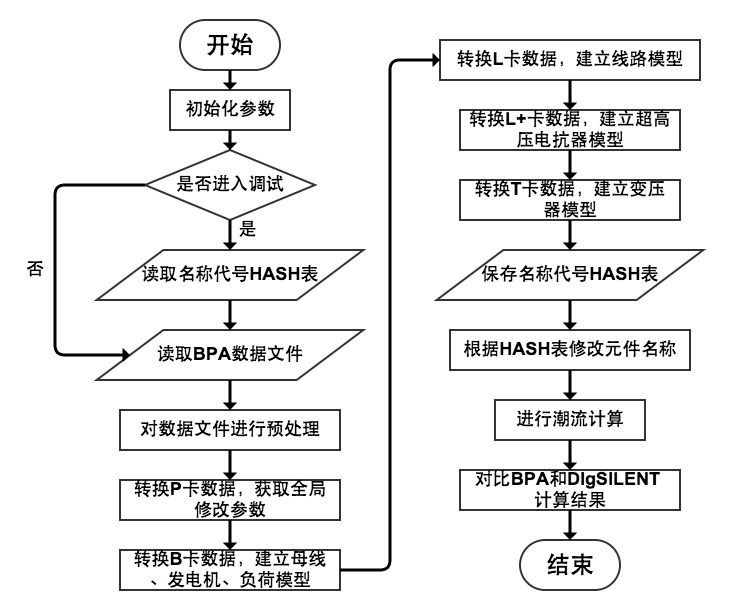
\includegraphics[width=1.05\textwidth]{images/Paper_Fig_12.png}
\setcaptionwidth{\linewidth}
\caption{BPA至DIgSILENT数据转换程序流程图}
\end{figure}

如图3.1所示为程序的运行流程图,BPA 模型导入 DIgSILENT 主要需要以下步骤:
  \begin{enumerate}[1)]
  \item 首先读取潮流修改卡片P卡,获取全网或部分网络发电出力或负荷的修改百分数。
  \item 建立母线、发电机和负荷节点的DIgSILENT模型,读取节点数据卡B卡,根据不同情况处理填入数据。
  \item 通过读取对称线路数据卡L卡和线路高抗参数数据卡L+卡,建立普通线路模型和超高压电抗器模型。
  \item 读取变压器数据卡T卡建立变压器模型。
  \item 在 DIgSILENT 和BPA中分别进行潮流计算,比较相关运行结果。
  \end{enumerate}

\section{论文的进度安排}

本文的主要内容是通过文献资料的阅读整理,学习数据转换的基础理论知识,了解有关的常规算法以及新提出的改进算法,研究这些算法的理论并且对目前常用的算法进行收集整理,分析各种算法的优缺点以及适用条件。认识并熟悉BPA和DIgSILENT的基本使用技巧,了解他们的数据格式,编程语言,并能有一定应用。

进度安排

3月23日-4月20日:进行文献资料的阅读学习,学习软件编程语言和仿真软件,研究由BPA到PSS/E的实现程序和董炜学长编写的BPA到DIgSILENT转换程序,熟悉软件使用;

4月21日-5月10日:进行程序的开发和调试;

5月11日-5月21日:结合算例对比程序运行结果,改进程序;

5月22日-结题:完成毕业论文的撰写。


